\documentclass[11pt]{article}
\usepackage[margin=1in]{geometry}
\usepackage{amsmath,amssymb,booktabs,hyperref}
\usepackage{pgfplots}\pgfplotsset{compat=1.18}
\usepackage[numbers,sort&compress]{natbib}
\title{Calibration Collapse Under the Homology Cliff: Distant-Stratum Precision of 0.068 and ECE of 0.294 in Frozen ESM-2 Retrieval}
\author{Santiago Maniches\thanks{ORCID 0009-0005-6480-1987. TOPOLOGICA LLC.}}
\date{April 12, 2026 (v1.1; erratum 2026-06-15, v1.2)}
\begin{document}\maketitle
\begin{abstract}
Beyond the $F_1$ cliff characterized in Paper 1, frozen ESM-2 \cite{lin2023evolutionary} cosine $k$-NN retrieval on our 24{,}885-protein biosecurity test set exhibits a severe calibration collapse across strata. Expected Calibration Error (ECE \cite{guo2017calibration}, six-bin reliability scheme) rises 4.3$\times$ from close-stratum 0.069 to distant-stratum 0.294. Distant-stratum positive-prediction precision drops to $3/44 = 0.068$: of 44 distant queries where the classifier predicts positive, only 3 are actually positive. In the highest-confidence bin ($[0.9, 1.0]$ of vote fraction), close-stratum empirical positive rate is 0.91 while distant-stratum empirical positive rate is 0.00 (3 predictions, 0 correct). The classifier is most confident where it is least accurate on this stratum. The distant stratum is a natural covariate-shift regime, and Ovadia et al. \cite{ovadia2019shift} previously documented that standard deep-classifier post-hoc calibration techniques lose their guarantees under such shift; we measure but do not test those rescues here. Deployment consequence: in our regime, every distant-stratum positive prediction requires human review regardless of vote count, and distant-stratum positive outputs are not safely usable as automated triggers. Temperature scaling and isotonic regression \cite{guo2017calibration} as post-hoc rescues are deferred to a follow-up. Headline values are committed as \texttt{data/results\_summaries/calibration\_results.json} and reproducible via \texttt{code/analyses/run\_calibration.py}.
\end{abstract}

\paragraph{Erratum (2026-06-15, v1.2).} The committed \texttt{calibration\_results.json} that fed this paper predated a panel-construction change and did not reproduce from the current, verified pipeline; it has been regenerated. Corrected close/moderate positive-prediction precision are \textbf{0.788} and \textbf{0.347} (previously 0.891 and 0.467); close/moderate stratum sizes are \textbf{22{,}198} and \textbf{1{,}533} (previously 22{,}090 and 1{,}641); and the reliability figure is now plotted from the script-computed reliability table rather than hand-entered diagram read-offs. The headline distant-stratum precision ($3/44 = 0.068$), all three ECE values (0.069 / 0.154 / 0.294), and every conclusion are unchanged. See \texttt{CHANGELOG.md}.

\section{Setup}
Analysis at t30 $R=1000$ $k=25$ cosine, seed 20260410 (seed chosen before calibration analysis, from the main pre-reg). Vote fraction: $\hat{p}(y=1) = \text{pos\_votes}/k$. Prediction: $\hat{y} = \mathbb{1}[\text{pos\_votes} \cdot 2 \ge k]$. Reliability binning: 6 bins at 0.1, 0.3, 0.5, 0.7, 0.9, 1.0. ECE = $\sum_b (|B_b|/n) \cdot |\text{acc}(B_b) - \text{conf}(B_b)|$.

\section{Results}
\begin{center}\small
\begin{tabular}{lrrr}
\toprule
stratum & $n$ & ECE & positive-prediction precision \\
\midrule
close ($s_{\max} \ge 0.95$) & 22{,}198 & 0.069 & 0.788 \\
moderate ($[0.90, 0.95)$) & 1{,}533 & 0.154 & 0.347 \\
distant ($< 0.90$) & 154 & \textbf{0.294} & \textbf{0.068} \\
\bottomrule
\end{tabular}\end{center}

Positive-prediction precision on distant stratum: 3 true positives out of 44 positive predictions. False alarm rate 41/44 = 93.2\% among distant positive predictions.

\begin{figure}[h]\centering
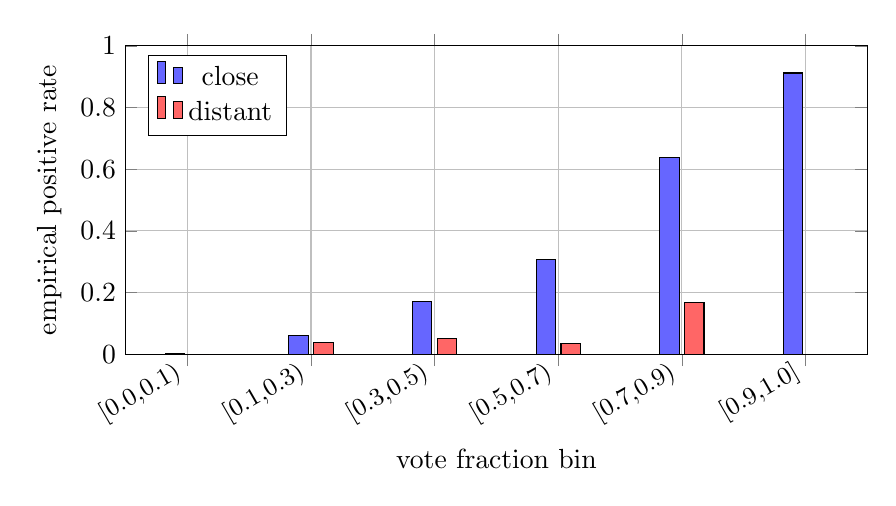
\begin{tikzpicture}\begin{axis}[width=11cm,height=5.5cm,xlabel={vote fraction bin},ylabel={empirical positive rate},ybar,bar width=7pt,grid=major,legend pos=north west,ymin=0,ymax=1,symbolic x coords={{[0.0,0.1)},{[0.1,0.3)},{[0.3,0.5)},{[0.5,0.7)},{[0.7,0.9)},{[0.9,1.0]}},xtick=data,x tick label style={rotate=30,anchor=east,font=\small}]
\addplot[fill=blue!60] coordinates {({[0.0,0.1)},0.003)({[0.1,0.3)},0.060)({[0.3,0.5)},0.171)({[0.5,0.7)},0.308)({[0.7,0.9)},0.637)({[0.9,1.0]},0.912)}; \addlegendentry{close}
\addplot[fill=red!60] coordinates {({[0.0,0.1)},0.000)({[0.1,0.3)},0.037)({[0.3,0.5)},0.051)({[0.5,0.7)},0.034)({[0.7,0.9)},0.167)({[0.9,1.0]},0.000)}; \addlegendentry{distant}
\end{axis}\end{tikzpicture}
\caption{Close-stratum reliability rises with confidence and is well-calibrated in aggregate (ECE 0.069). Distant-stratum reliability is flat across confidence bins and collapses in the highest-confidence bin (3 predictions, 0 correct; ECE 0.294). Bars are the script-computed empirical positive rate per bin.}
\end{figure}

\section{Why this matters}
In biosecurity deployment, downstream filters often gate on vote-fraction confidence: route high-confidence positives to automated action, route low-confidence to review. Under the cliff, this policy fails catastrophically on the distant stratum: the single highest-confidence bin contains 3 predictions, all wrong, while adjacent lower-confidence bins have higher empirical rates. Confidence ranking within the distant stratum is essentially noise.

\section{Related: calibration under distribution shift}
Ovadia et al. \cite{ovadia2019shift} showed standard deep-classifier calibration methods (temperature scaling \cite{guo2017calibration}, deep ensembles) lose their guarantees under covariate shift. Our distant stratum is a natural covariate-shift regime induced by embedding-space distance from the panel. The standard correction family \cite{guo2017calibration} does not straightforwardly apply because the shift is unbounded along the $s_{\max} < 0.90$ ray. Temperature scaling \cite{guo2017calibration} and isotonic regression \cite{guo2017calibration} are natural next-pass rescues, deferred. Panel augmentation is disfavored by the cross-family result in the companion Paper 5 (Wilson 95\% CI on within-family rate $[0\%, 17\%]$); post-hoc distance substitution is rejected at pre-registered H1 by Paper 2 \cite{ledoit2004,amari2016,weinberger2009distance,schroff2015facenet,lin2023evolutionary}.

\section{Limitations}
(L1) Single-seed analysis; 10-seed extension deferred. (L2) ECE is known to be sensitive to binning; we report a six-bin scheme with boundaries $\{0.0, 0.1, 0.3, 0.5, 0.7, 0.9, 1.0\}$ (tight tails, wide middle), per the locked binning in \texttt{code/analyses/run\_calibration.py}. Re-binning may shift the absolute ECE values. (L3) Calibration under the learned-projection rescue (Paper 1) unmeasured. (L4) Isotonic regression and Platt scaling as post-hoc rescues untested.

\bibliographystyle{unsrtnat}\bibliography{references}\end{document}
